\chapter{CNN Building Blocks}
\label{ch:blocks}

\chapmeta{Beginner}{$\sim$4\,h (2\,h theory + 2\,h practical)}{EuroSAT; synthetic data}

\begin{objbox}
\begin{itemize}[leftmargin=1.2em,nosep]
  \item Understand pooling (max/average) and global pooling, and their effect on resolution.
  \item Compare activation functions and know when to use each.
  \item Explain batch normalisation and why it stabilises and accelerates training.
  \item Use dropout to regularise, and recognise the signature of overfitting.
  \item Assemble these into a complete, well-reasoned CNN classifier.
\end{itemize}
\end{objbox}

A convolution layer alone is a linear operator. A working CNN interleaves it
with non-linearities, downsampling, normalisation and regularisation. This
chapter covers those building blocks and assembles them into the
\texttt{SimpleCNN} we train in Chapter~\ref{ch:classif}.

\section{Pooling}

Pooling downsamples a feature map, reducing spatial resolution (and therefore
computation) while enlarging the effective receptive field. \emph{Max pooling}
takes the maximum over each $p\times p$ window; \emph{average pooling} takes the
mean (Figure~\ref{fig:pool}):
\begin{equation}
\mathrm{MaxPool}(X)[i,j]=\!\!\max_{0\le m,n<p}\! X[si+m,\,sj+n],\quad
\mathrm{AvgPool}(X)[i,j]=\frac{1}{p^2}\!\sum_{m,n} X[si+m,\,sj+n].
\end{equation}
Max pooling preserves the strongest activation (good for detecting whether a
feature is \emph{present}); average pooling smooths. Most modern networks use
strided convolutions or max pooling in the body and a \emph{global average
pool} (GAP) at the end, collapsing each $C\times H\times W$ feature map to a
$C$-vector by averaging over space. GAP removes the need for large fully
connected layers, drastically cutting parameters and overfitting, and underlies
class-activation maps (Chapter~\ref{ch:eval}).

\begin{figure}[h]
\centering
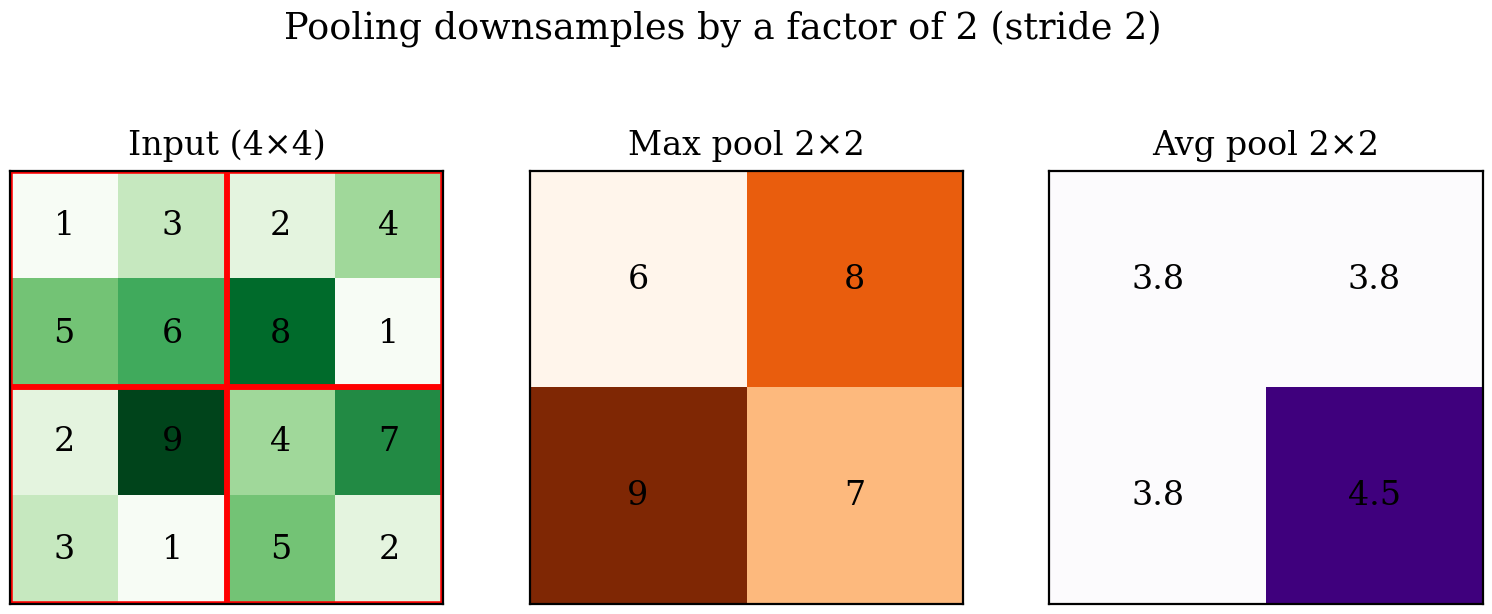
\includegraphics[width=0.92\linewidth]{figures/pooling.png}
\caption{Max vs average pooling with a $2\times2$ window and stride 2. Both halve
each spatial dimension; max pooling keeps the dominant response, average pooling
the local mean.}
\label{fig:pool}
\end{figure}

\section{Activation functions}

Without a non-linearity, a stack of convolutions collapses to a single linear
map. The activation $\phi$ applied element-wise after each layer gives the
network its expressive power (Figure~\ref{fig:act}). The default is the
rectified linear unit:
\begin{equation}
\mathrm{ReLU}(z)=\max(0,z).
\end{equation}
ReLU is cheap, non-saturating for $z>0$, and induces sparsity, but ``dead''
units can occur when a neuron is pushed permanently negative.
\emph{LeakyReLU}, $\phi(z)=\max(\alpha z,z)$ with small $\alpha$, keeps a
gradient for $z<0$. \emph{GELU}, $\phi(z)=z\,\Phi(z)$ (with $\Phi$ the Gaussian
CDF), is a smooth variant favoured in transformers. The saturating
\emph{sigmoid} $\sigma(z)=1/(1+e^{-z})$ and \emph{tanh} are now used mainly in
output layers (binary probability) or gates, because their vanishing gradients
slow deep training.

\begin{figure}[h]
\centering
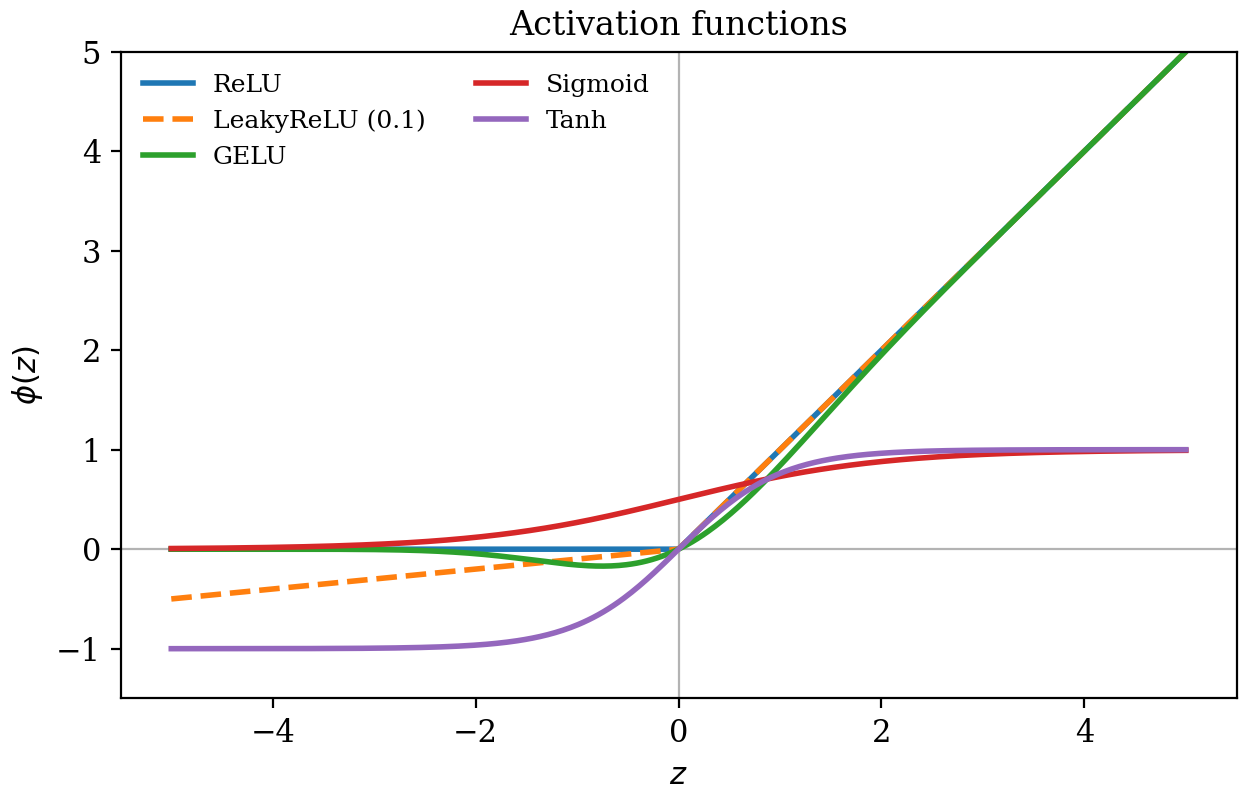
\includegraphics[width=0.68\linewidth]{figures/activations.png}
\caption{Common activation functions. ReLU and its smooth relatives (LeakyReLU,
GELU) dominate hidden layers; sigmoid/tanh saturate and are reserved for outputs
and gates.}
\label{fig:act}
\end{figure}

\section{Batch normalisation}

Batch normalisation (Ioffe \& Szegedy, 2015) normalises each channel's
pre-activations across the mini-batch, then rescales with learnable parameters
$\gamma,\beta$. For a channel with batch values $\{x_i\}$:
\begin{align}
\mu_B &= \frac1m\sum_i x_i, &
\sigma_B^2 &= \frac1m\sum_i (x_i-\mu_B)^2,\\
\hat x_i &= \frac{x_i-\mu_B}{\sqrt{\sigma_B^2+\epsilon}}, &
y_i &= \gamma\,\hat x_i + \beta.
\label{eq:bn}
\end{align}
BatchNorm reduces \emph{internal covariate shift}, smooths the loss landscape,
permits higher learning rates, and acts as a mild regulariser. At inference it
uses running estimates of $\mu,\sigma$ accumulated during training. Because BN
already provides a per-channel shift $\beta$, the preceding convolution sets
\texttt{bias=False}. Place it as \texttt{Conv $\to$ BN $\to$ ReLU}.

\begin{notebox}[Small-batch caveat]
BatchNorm statistics are unreliable with very small batches (common for
high-resolution segmentation on limited VRAM). In that regime prefer GroupNorm
or InstanceNorm, which normalise without a batch dependency.
\end{notebox}

\section{Dropout and overfitting}

Overfitting occurs when a model memorises training data and fails to generalise;
its signature is a training loss that keeps falling while validation loss rises.
\emph{Dropout} (Srivastava et al., 2014) combats this by randomly zeroing a
fraction $p$ of activations during training, scaling the survivors by
$1/(1-p)$, which prevents co-adaptation and approximates an ensemble. It is
disabled at inference. In convolutional bodies dropout is used sparingly
(spatial structure makes element-wise dropout weak); it is most effective in
the dense head. The stronger regularisers for CNNs are data augmentation
(Chapter~\ref{ch:aug}), weight decay, and BatchNorm itself.

\section{Assembling a CNN}

A canonical small classifier stacks \emph{blocks} of
\texttt{Conv$\to$BN$\to$ReLU$\to$Pool}, doubling channels as resolution halves,
then a GAP and a linear classifier:
\begin{lstlisting}
import torch.nn as nn
class ConvBlock(nn.Module):
    def __init__(self, cin, cout):
        super().__init__()
        self.net = nn.Sequential(
            nn.Conv2d(cin, cout, 3, padding=1, bias=False),
            nn.BatchNorm2d(cout), nn.ReLU(inplace=True),
            nn.MaxPool2d(2))            # halves H, W
    def forward(self, x): return self.net(x)

class SimpleCNN(nn.Module):
    def __init__(self, in_ch=3, n_classes=10):
        super().__init__()
        self.features = nn.Sequential(
            ConvBlock(in_ch, 32),       # 64 -> 32
            ConvBlock(32, 64),          # 32 -> 16
            ConvBlock(64, 128))         # 16 -> 8
        self.head = nn.Sequential(
            nn.AdaptiveAvgPool2d(1), nn.Flatten(),
            nn.Dropout(0.3), nn.Linear(128, n_classes))
    def forward(self, x): return self.head(self.features(x))
\end{lstlisting}
The channel-doubling/resolution-halving rule keeps the per-layer compute roughly
constant while building an increasingly abstract, lower-resolution
representation --- a pattern you will see again in every ResNet and U-Net
encoder.

\begin{keybox}
\begin{itemize}[leftmargin=1.2em,nosep]
  \item Pooling/strides downsample and grow the RF; GAP replaces heavy FC heads.
  \item ReLU is the default hidden activation; sigmoid/tanh for outputs/gates.
  \item BatchNorm (Eq.~\ref{eq:bn}) stabilises and speeds training; order is Conv$\to$BN$\to$ReLU, bias off.
  \item Overfitting $=$ train loss $\downarrow$ while val loss $\uparrow$; fight it with augmentation, weight decay, dropout.
  \item Standard pattern: blocks of Conv-BN-ReLU-Pool, doubling channels, then GAP + linear.
\end{itemize}
\end{keybox}

\begin{practbox}
Notebook: \nbpath{chapter\_03\_cnn\_building\_blocks/03\_practical\_cnn\_components.ipynb}.
\begin{enumerate}[leftmargin=1.4em,nosep]
  \item Visually compare max vs average pooling on a sample feature map.
  \item Plot ReLU, LeakyReLU, GELU, sigmoid and tanh and their gradients.
  \item Train a small net \emph{with} and \emph{without} BatchNorm; compare loss
  curves and the largest stable learning rate.
  \item Force overfitting on a tiny subset, then add dropout and observe the
  validation-loss gap shrink.
  \item Build \texttt{SimpleCNN}; print a layer-by-layer summary of shapes and
  parameter counts.
\end{enumerate}
\end{practbox}

\begin{exbox}
\textbf{3.1 Architecture ablation.} Vary depth (2 vs 3 vs 4 blocks) and width
(16/32/64 base channels); tabulate parameters, train time and accuracy.\\[2pt]
\textbf{3.2 Normalisation swap.} Replace BatchNorm with GroupNorm; retrain at
batch size 4 and explain the difference.\\[2pt]
\textbf{3.3 Activation study.} Swap ReLU for LeakyReLU and GELU; measure
convergence speed and final accuracy.\\[2pt]
\textbf{Mini-project.} Implement a configurable \texttt{make\_cnn(depth, width,
norm, act, dropout)} factory and run a small grid search on EuroSAT, reporting a
parameters-vs-accuracy scatter plot.
\end{exbox}
